% Principally, this chapter should describe the work which was undertaken before code was written, hardware built
% or theories worked on. It should show how the project proposal was further refined and clarified, so that the
% Implementation stage could go smoothly rather than by trial and error.

% Throughout this chapter and indeed the whole dissertation, it is essential to demonstrate that a proper 
% professional approach was employed.

% The nature of this chapter will vary greatly from one dissertation to another but, underlining the professional 
% approach, this chapter will very likely include a section headed “Requirements Analysis” and incorporate other 
% references to software engineering techniques.

% The chapter will cite any new programming languages and systems which had to be learnt and will mention 
% complicated theories or algorithms which required understanding.

% It is essential to declare the Starting Point (see Section 7). This states any existing codebase or materials 
% that your project builds on. The text here can commonly be identical to the text in your proposal, but it may 
% enlarge on it or report variations. For instance, the true starting point may have turned out to be different 
% from that declared in the proposal and such discrepancies must be explained.

% ~2500 words

\documentclass[final,dissertation.tex]{subfiles}
\begin{document}

\chapter{Preparation (Due 20th April)}

This chapter begins by providing a high level overview of how Loopix is structured, ......

\section{Structure of Loopix (Due 23rd March)}

In this section, I describe the Loopix network architecture, and the Poisson Mix theory. An overview of the network architecture is shown in Figure~\ref{fig:loopix_network}. 

\subsection{Network Architecture}

\begin{figure}[h]
	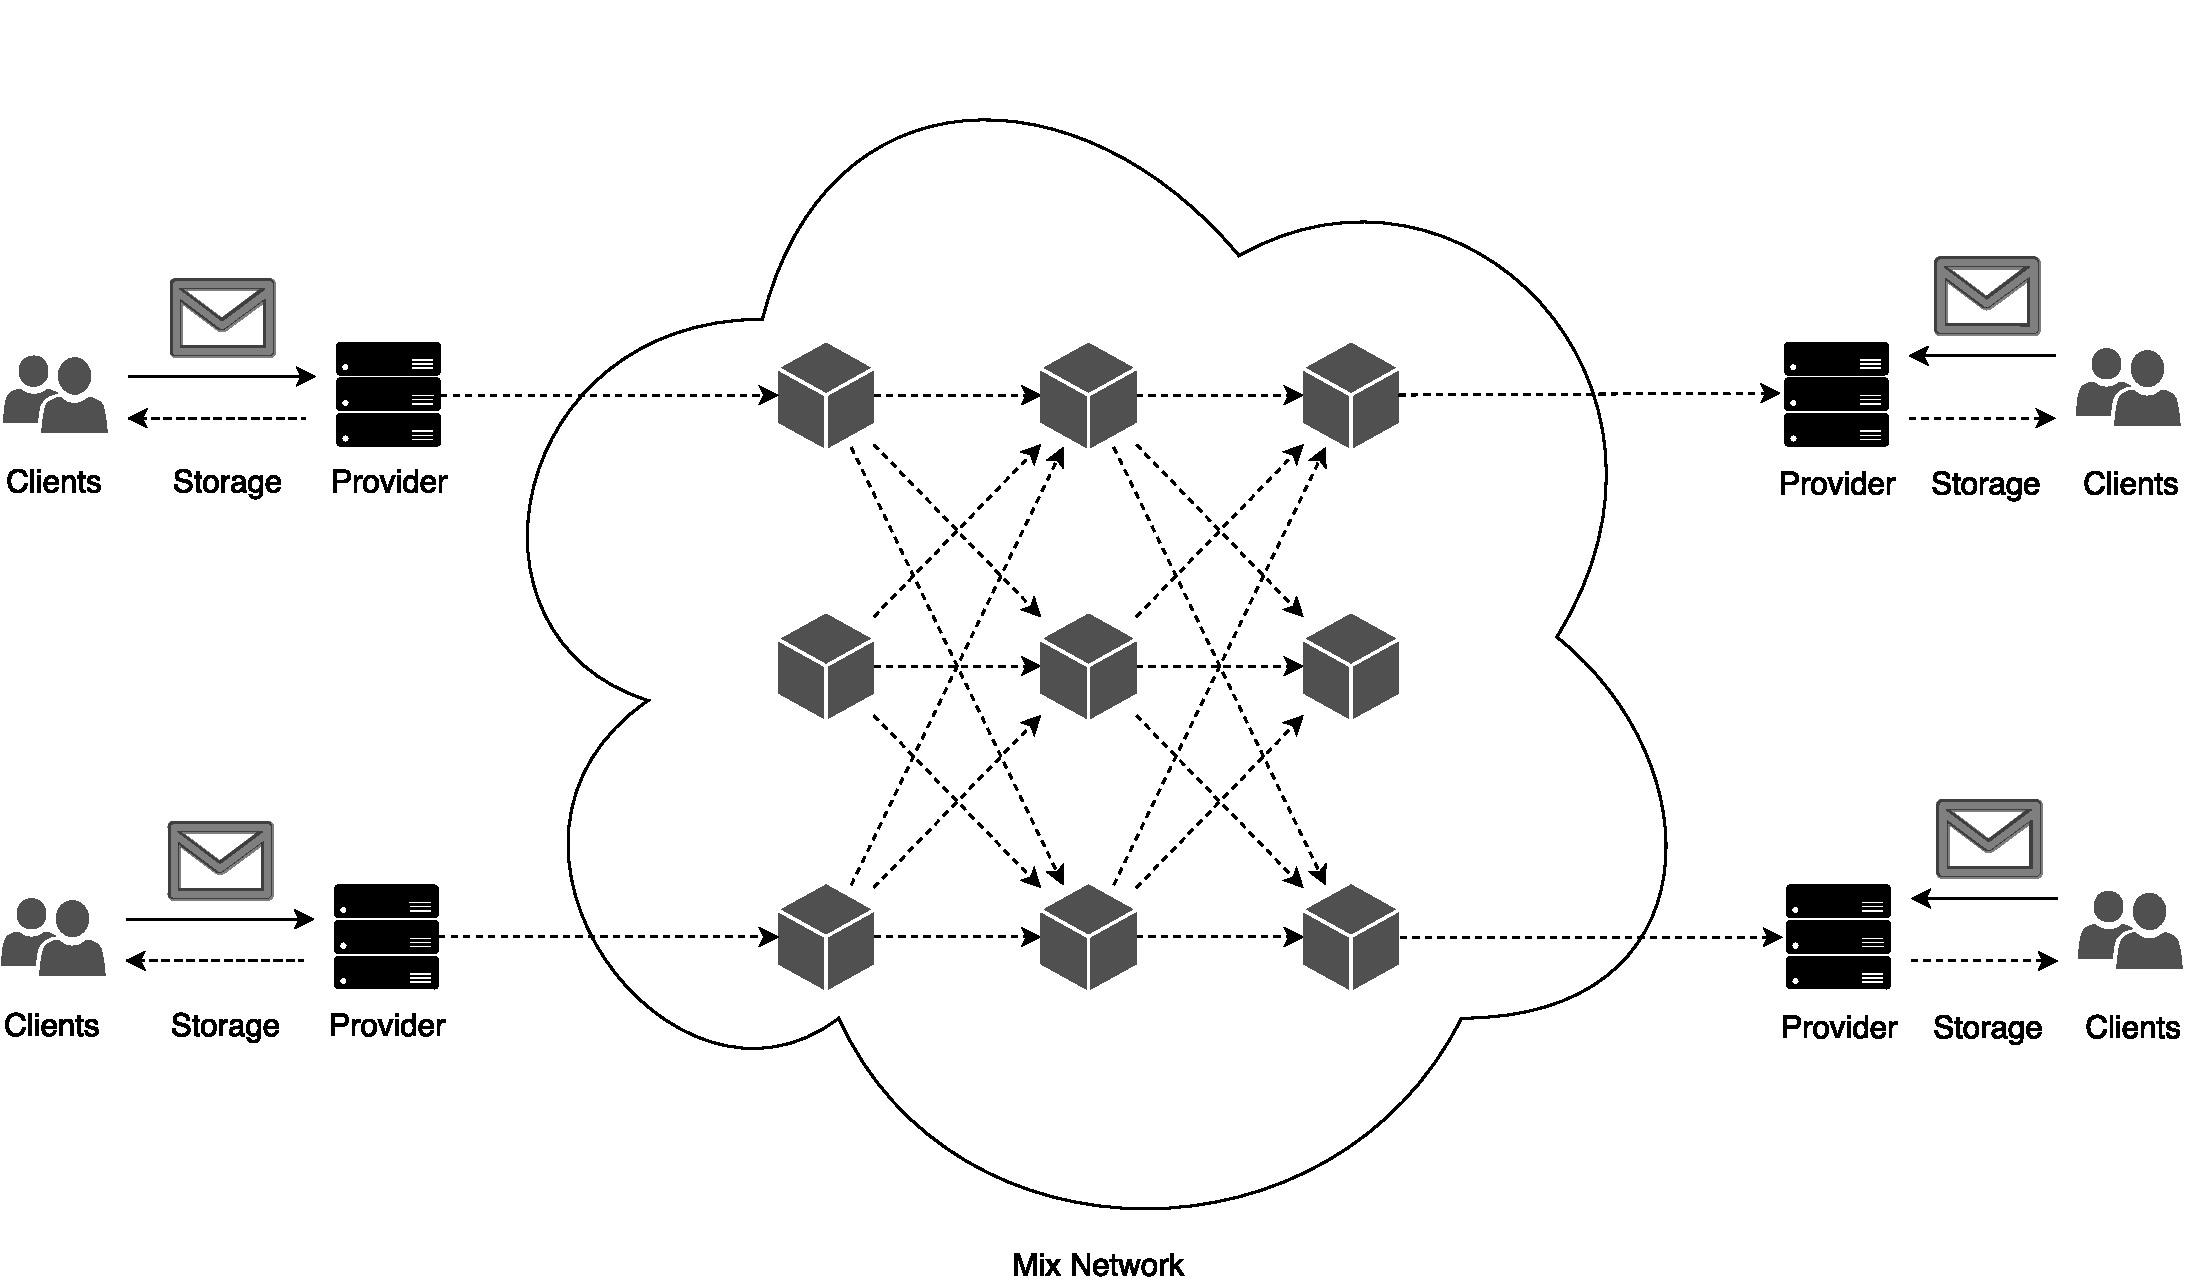
\includegraphics[width=\linewidth]{../figs/loopix_network}
	\caption{Overview of the Loopix network architecture. Clients pass messages to their providers, which are responsible for injecting the message into the mix network. The received messages are stored in inboxes at providers and retrieved by clients when they come online. TODO: Refine the figure with message paths }\label{fig:loopix_network}
\end{figure}

The Loopix network is composed of three parts: clients, mix nodes and providers. A client can communicate through the Loopix network and can act as a sender and receiver of messages. Each entity in the Loopix network has a unique public-private key pair that is used to encrypt and decrypt messages. The mix nodes are separated into layers, with each layer forwarding messages to the next layer. 

In order for a sender to send a message to a receiver, the sender needs to know the receiver's Loopix network location, that is the IP address of the receiver's provider, an identifier of the user, and the receiver's public encryption key. The sender also needs to know the network locations of intermediate mix nodes as the sender is responsible for selecting the route through the network.


\subsection{Poisson Mix}

Loopix employs a strategy called the Poisson Mix to prevent observers from learning the correspondences between incoming and outgoing messages at a node, therefore guarding against a global passive adversary performing traffic analysis attacks. 

When a mix packet arrives at a mix node, the mix node decodes and extracts the subsequent mix packet to forward on. The decoded message includes a delay parameter which specifies how long to delay the forwarding of the packet. This delay parameter is determined by the source of the message. Honest clients choose this delay by sampling from an exponential distribution with a parameter $\lambda$ that is assumed to be public and the same for all mix nodes.

Since honest nodes generate cover traffic, loop traffic, and real traffic following a Poisson process, aggregating these traffic streams at the input of a mix node produces another Poisson process with a rate $\lambda_m$ dependent on the number of mix nodes and clients.

As this input process is a Poisson process, and each message is independently delayed using an exponential distribution with parameter $\lambda$, a Poisson Mix can be modelled as an $M/M/\infty$ queueing system since both input and output of the mix node are Poisson processes. As a result of the memoryless property of such a system, messages are indistinguishable from each other, since messages are emitted with equal probability regardless of the amount of time they have been waiting in the queue.

\section{Cryptography}

\subsection{Elliptic Curves}

\subsection{LIONESS Wide Cipher}

\section{Requirements Analysis}

Sphinx, Loopix, Testnet, Evaluation

\section{Development Tools}

IDEA IntelliJ

Docker

\section{Existing Libraries}

\subsection{Python Loopix Library}

\subsection{Bouncy Castle}
\label{sec:bouncy}

Crypto (AES/SHA/HMAC/ECC)

Chosen for easier portability between clients which may not have the official java crypto extension installed, or have the neccessary ciphers.

\section{Software Engineering Techniques}

Test driven development. Existing library allows generation of test data to verify correctness and compatibility.

\end{document}